\documentclass{article}
\usepackage[utf8]{inputenc}
\usepackage{amsmath}
\usepackage{amssymb}
\usepackage{geometry}
\usepackage{graphicx}
\usepackage{float}
\usepackage{tikz}
\usepackage{graphicx}   
\usepackage{subcaption} 
\usetikzlibrary{shapes.geometric, arrows, positioning, calc, patterns}

\geometry{a4paper, margin=1in}

\title{Model Extension: Author-Journal Game with Competition and Capacity Constraints}

\date{\today}

\begin{document}

\maketitle

\section{Motivation and Problem Statement}

In our previous evolutionary game-theoretic model of the author-journal interaction, we observed that the equilibrium strategies were largely insensitive to the population size $N$.
This phenomenon arises because, in the original formulation, the payoff of a focal author depends solely on their own strategy and the journal's acceptance policy, but is independent of the actions of other authors.
Consequently, there is no \textit{congestion effect} or \textit{competition} for limited resources.
To address this and model a more realistic academic publishing environment (e.g., conferences with fixed acceptance rates or journals with limited pages), we introduce a capacity threshold $K$.
This mechanism creates a zero-sum element: as the number of submissions increases, the probability of acceptance for a passed paper decreases, potentially disincentivizing opportunistic strategies like \textit{Always Submit} (AS).

\section{The Threshold Competition Model}

The updated interaction proceeds in the following stages:
\begin{enumerate}
    \item \textbf{Submission:} $N$ authors choose a strategy $s \in \{\text{OG}, \text{AS}, \dots\}$.
    \item \textbf{Peer Review (Perception):} All submissions undergo peer review characterized by false negative rate $\epsilon$ and false positive rate $\lambda$.
    Papers that pass peer review enter a ``Perception Pool'' of size $M$.
    \item \textbf{Competition (Threshold Cut):} The journal has a maximum capacity $K$.
    \begin{itemize}
        \item If $M \le K$, all papers in the pool are accepted.
        \item If $M > K$, the journal randomly selects $K$ papers from the pool to accept.
        The remaining $M-K$ papers are rejected despite passing review.
    \end{itemize}
\end{enumerate}


Let $\alpha$ be the probability an author produces a good paper.
The probability that a single author's submission passes the peer review stage, denoted as $P_{pass}(s)$, depends on their chosen strategy $s$:

\begin{align}
    P_{pass}(\text{OG}) &= \alpha(1-\epsilon) \\
    P_{pass}(\text{AS}) &= \alpha(1-\epsilon) + (1-\alpha)\lambda
\end{align}

Here, OG authors only submit good papers, while AS authors submit both good and bad papers, benefiting from the false positive rate $\lambda$.

\begin{figure}[htbp]
    \centering
    \resizebox{\textwidth}{!}{
        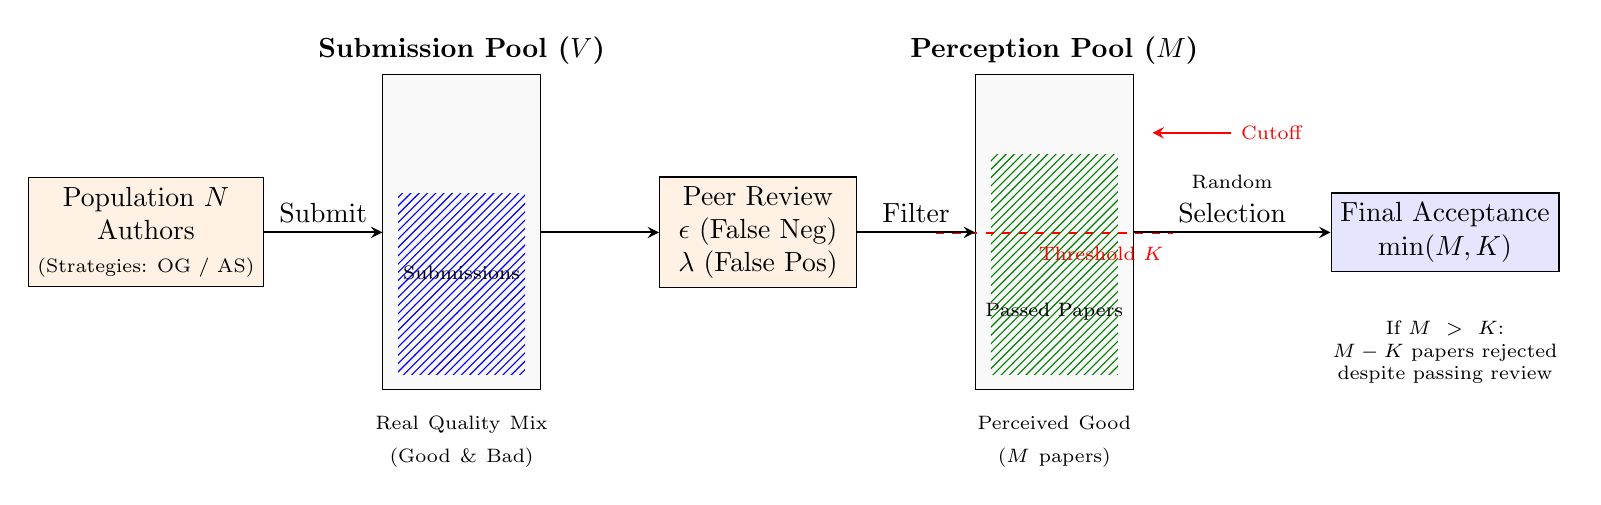
\begin{tikzpicture}[node distance=2cm, auto, >=stealth]

        % --- Styles ---
        \tikzstyle{process} = [rectangle, minimum width=2.5cm, minimum height=1cm, text centered, draw=black, fill=orange!10]
        \tikzstyle{pool} = [rectangle, minimum width=2cm, minimum height=4cm, draw=black, fill=gray!5]
        \tikzstyle{arrow} = [thick,->]

        % --- Nodes ---

        % 1. Authors
        \node (authors) [process, align=center] {Population $N$ \\ Authors \\ \scriptsize (Strategies: OG / AS)};
        
        % 2. Submission Pool (UPDATED: S -> V)
        \node (submit_pool) [pool, right=1.5cm of authors, label=above:\textbf{Submission Pool ($V$)}] {};
        \fill[pattern=north east lines, pattern color=blue] ($(submit_pool.south west) + (0.2,0.2)$) rectangle ($(submit_pool.south east) + (-0.2, 2.5)$);
        \node at ($(submit_pool.south) + (0, 1.5)$) {\scriptsize Submissions};

        % 3. Peer Review
        \node (review) [process, right=1.5cm of submit_pool, align=center] {Peer Review \\ $\epsilon$ (False Neg) \\ $\lambda$ (False Pos)};
        
        % 4. Perception Pool
        \node (percep_pool) [pool, right=1.5cm of review, label=above:\textbf{Perception Pool ($M$)}] {};
        \fill[pattern=north east lines, pattern color=green!50!black] ($(percep_pool.south west) + (0.2,0.2)$) rectangle ($(percep_pool.south east) + (-0.2, 3.0)$);
        \node at ($(percep_pool.south) + (0, 1.0)$) {\scriptsize Passed Papers};

        % --- Threshold K ---
        \draw[red, thick, dashed] ($(percep_pool.south west) + (-0.5, 2.0)$) -- ($(percep_pool.south east) + (0.5, 2.0)$);
        \node[text=red, anchor=north east, yshift=-0.05cm] at ($(percep_pool.south east) + (0.5, 2.0)$) {\scriptsize Threshold $K$};
        
        % 5. Final Selection
        \node (final) [process, right=2.5cm of percep_pool, align=center, fill=blue!10] {Final Acceptance \\ $\min(M, K)$};
        
        % --- Arrows ---
        \draw[arrow] (authors) -- node[above] {Submit} (submit_pool);
        \draw[arrow] (submit_pool) -- (review);
        \draw[arrow] (review) -- node[above] {Filter} (percep_pool);
        \draw[arrow] (percep_pool) -- node[above, align=center] (rand_sel) {\scriptsize Random\\Selection} (final);
        
        % Label and Cutoff Arrow
        \node[above=0.2cm of rand_sel, xshift=0.5cm, text=red] (cutoff_label) {\scriptsize Cutoff};
        \draw[->, red, thick] (cutoff_label.west) -- ++(-1.0, 0);
        
        % --- Footnotes ---
        \node [below=0.2cm of submit_pool, text width=2.5cm, align=center] {\scriptsize Real Quality Mix\\(Good \& Bad)};
        \node [below=0.2cm of percep_pool, text width=2.5cm, align=center] {\scriptsize Perceived Good\\($M$ papers)};
        \node [below=0.5cm of final, text width=3cm, align=center, font=\scriptsize] {If $M > K$: \\ $M-K$ papers rejected \\ despite passing review};
        \end{tikzpicture}
    }
    \caption{\textbf{Schematic representation of the Threshold Competition Model.} The process unfolds in three stages: (1) Submission into a pool $V$;
    (2) Peer review filtering into a perception pool $M$; and (3) A hard capacity constraint $K$ (red dashed line).
    If $M > K$, a random cutoff occurs, rejecting surplus papers even if they passed review.
    This introduces the rationing probability $\rho$.}
    \label{fig:threshold_model}
\end{figure}

\section{Derivation of the Rationing Probability $\rho$}

The key addition to the payoff function is the rationing probability $\rho$, which represents the probability that a paper is finally accepted \textit{given that it has already passed peer review}.
Let us consider a \textit{focal author} who has passed peer review.
Let $M_{-i}$ be the random variable representing the number of \textit{other} authors (out of $N-1$) whose papers also passed peer review.
The total number of passed papers is therefore $M = 1 + M_{-i}$.
The rationing probability for the focal author is defined as:
\begin{equation}
    \rho_{\text{focal}} = \min\left(1, \frac{K}{1 + M_{-i}}\right) = 
    \begin{cases} 
      1 & \text{if } 1 + M_{-i} \le K \\
      \frac{K}{1 + M_{-i}} & \text{if } 1 + M_{-i} > K
   \end{cases}
\end{equation}

\subsection{Expected Rationing Probability}
Since $M_{-i}$ is a random variable, authors base their decisions on the expected value $E[\rho_{\text{focal}}]$.
Assume the population consists of $N_{\text{OG}}$ authors playing OG and $N_{\text{AS}}$ authors playing AS (where $N_{\text{OG}} + N_{\text{AS}} = N - 1$, excluding the focal author).
The variable $M_{-i}$ is the sum of two independent binomial distributions:
\begin{equation}
    M_{-i} = X_{\text{OG}} + X_{\text{AS}}
\end{equation}
where $X_{\text{OG}} \sim B(N_{\text{OG}}, P_{pass}(\text{OG}))$ and $X_{\text{AS}} \sim B(N_{\text{AS}}, P_{pass}(\text{AS}))$.
The expected rationing probability is given by:
\begin{equation}
    E[\rho_{\text{focal}}] = \sum_{m=0}^{N-1} \Pr(M_{-i} = m) \cdot \min\left(1, \frac{K}{1 + m}\right)
\end{equation}


\section{Payoff after competition}

In this section, we rigorously define the payoff functions for both authors and journals under the Threshold Competition Model.
The introduction of the capacity constraint $K$ and the endogenous rationing probability $\rho$ fundamentally alters the strategic landscape.
We first define the key variables used in the payoff derivation:

\begin{table}[h]
\centering
\begin{tabular}{cl}
\hline
\textbf{Symbol} & \textbf{Description} \\ \hline
$N$ & Total number of authors \\
$K$ & Journal capacity (maximum number of accepted papers) \\
$V$ & Total number of submissions (Submission Pool) \\
$M$ & Number of papers passing peer review (Perception Pool) \\
$\rho$ & Rationing probability, probability of acceptance after passing review \\
$\alpha$ & Probability that an author produces a good paper \\
$\epsilon$ & False negative rate (probability of rejecting a good paper) \\
$\lambda$ & False positive rate (probability of accepting a bad paper) \\
$r$ & Reward for an accepted paper (Author) \\
$c$ & Cost of submission (Author) \\
$B$ & Benefit for accepting a good paper (Journal) \\
$D$ & Penalty for accepting a bad paper (Journal) \\
$C(V)$ & Cost of reviewing $V$ submissions \\
\hline
\end{tabular}
\caption{Key notation and definitions.}
\label{tab:variables}
\end{table}

\subsection{Journal}

The journal's payoff is determined by the quality of the accepted papers minus the cost of reviewing.
The crucial addition in this model is that the rationing probability $\rho$ is endogenous to the journal's strategy.
The journal maximizes its utility by choosing a strategy $S_J \in \{\text{OG}, \text{AA}, \text{OB}, \text{AR}\}$.
The rationing probability $\rho$ is defined as the ratio of capacity $K$ to the size of the perception pool $M$, capped at 1:
\begin{equation}
    \rho(S_J) = \min\left(1, \frac{K}{M(S_J)}\right)
\end{equation}
Since the screening policy (determined by effective $\epsilon$ and $\lambda$) changes the size of $M$, $\rho$ varies across strategies.
Let $V_{good}$ and $V_{bad}$ be the total number of good and bad papers submitted by the authors, such that $V = V_{good} + V_{bad}$.

\paragraph{Only Good (OG) -- Selective Strategy}
The journal applies standard peer review to filter papers, aiming to accept good papers and reject bad ones.
\begin{itemize}
    \item \textbf{Screening parameters:} Standard $\epsilon$ and $\lambda$.
    \item \textbf{Perception Pool ($M_{\text{OG}}$):} Contains accepted good papers and falsely accepted bad papers.
    \begin{equation}
        M_{\text{OG}} = V_{good}(1-\epsilon) + V_{bad}\lambda
    \end{equation}
    \item \textbf{Rationing Probability ($\rho_{\text{OG}}$):}
    \begin{equation}
        \rho_{\text{OG}} = \min\left(1, \frac{K}{V_{good}(1-\epsilon) + V_{bad}\lambda}\right)
    \end{equation}
    \item \textbf{Payoff ($U_J(\text{OG})$):} The journal gains $B$ from good papers and loses $D$ from bad papers, scaled by $\rho_{\text{OG}}$.
    \begin{equation}
        U_J(\text{OG}) = \rho_{\text{OG}} \left[ B \cdot V_{good}(1-\epsilon) - D \cdot V_{bad}\lambda \right] - C(V)
    \end{equation}
\end{itemize}

\paragraph{Always Accept (AA) -- Permissive Strategy}
The journal abandons screening, effectively setting $\epsilon=0$ and $\lambda=1$.
\begin{itemize}
    \item \textbf{Perception Pool ($M_{\text{AA}}$):} All submissions enter the pool.
    \begin{equation}
        M_{\text{AA}} = V = V_{good} + V_{bad}
    \end{equation}
    \item \textbf{Rationing Probability ($\rho_{\text{AA}}$):} This strategy maximizes congestion.
    \begin{equation}
        \rho_{\text{AA}} = \min\left(1, \frac{K}{V}\right)
    \end{equation}
    \item \textbf{Payoff ($U_J(\text{AA})$):}
    \begin{equation}
        U_J(\text{AA}) = \rho_{\text{AA}} \left[ B \cdot V_{good} - D \cdot V_{bad} \right] - C(V)
    \end{equation}
\end{itemize}

\paragraph{Only Bad (OB) -- Irrational Strategy}
The journal adopts an inverse selection policy, accepting papers that are perceived as ``bad'' by the peer review process.
This strategy effectively targets papers that fail the standard quality threshold.
\begin{itemize}
    \item \textbf{Perception Pool ($M_{\text{OB}}$):} The pool consists of good papers that were falsely rejected (false negatives) and bad papers that were correctly identified as bad (true negatives).
    \begin{equation}
        M_{\text{OB}} = V_{good}\epsilon + V_{bad}(1-\lambda)
    \end{equation}
    \item \textbf{Rationing Probability ($\rho_{\text{OB}}$):}
    \begin{equation}
        \rho_{\text{OB}} = \min\left(1, \frac{K}{V_{good}\epsilon + V_{bad}(1-\lambda)}\right)
    \end{equation}
    \item \textbf{Payoff ($U_J(\text{OB})$):} Although the journal intends to select bad papers, it may accidentally accept good papers due to review errors ($\epsilon$).
    However, it also accepts the vast majority of bad papers.
    \begin{equation}
        U_J(\text{OB}) = \rho_{\text{OB}} \left[ B \cdot V_{good}\epsilon - D \cdot V_{bad}(1-\lambda) \right] - C(V)
    \end{equation}
    Note that despite the potential small gain from $B \cdot V_{good}\epsilon$, the term $-D \cdot V_{bad}(1-\lambda)$ typically dominates because $D > B$ and $(1-\lambda) \gg \epsilon$ in realistic settings.
    Thus, $U_J(\text{OB})$ remains strictly dominated by strategies that do not actively seek penalties.
\end{itemize}

\paragraph{Always Reject (AR) -- Baseline Strategy}
The journal rejects all submissions.
The perception pool is empty ($M=0$), and no papers are published.
\begin{itemize}
    \item \textbf{Payoff ($U_J(\text{AR})$):}
    \begin{equation}
        U_J(\text{AR}) = 0
    \end{equation}
\end{itemize}

\subsection{Author}

An author chooses a strategy $S_A \in \{\text{OG}, \text{OB}, \text{AS}, \text{NS}\}$.
The author's expected utility depends on the probability of producing a good paper ($\alpha$), the cost of submission ($c$), the reward ($r$), and the probability of acceptance.
The probability of acceptance is a two-step process: passing the peer review (denoted as $P_{pass}$) and surviving the competition cut (denoted by $\rho$).
The expected payoff is generally given by:
\begin{equation}
    U_A = P(\text{Good}) \cdot P(\text{Accept}|\text{Good}) \cdot r + P(\text{Bad}) \cdot P(\text{Accept}|\text{Bad}) \cdot r - \text{Total Cost}
\end{equation}

Assuming the journal plays the standard \textit{Only Good} strategy (implying the rationing probability is $\rho_{\text{OG}}$), the payoffs for the four author strategies are derived as follows:

\paragraph{Only Good (OG)}
The author submits only if the paper is good.
\begin{itemize}
    \item Probability of submission: $\alpha$
    \item Probability of passing review: $1-\epsilon$
    \item \textbf{Payoff:}
    \begin{equation}
        U_A(\text{OG}) = \alpha \left[ (1-\epsilon) \rho_{\text{OG}} r - c \right]
    \end{equation}
\end{itemize}

\paragraph{Only Bad (OB)}
The author submits only if the paper is bad, attempting to exploit the false positive rate.
\begin{itemize}
    \item Probability of submission: $1-\alpha$
    \item Probability of passing review: $\lambda$
    \item \textbf{Payoff:}
    \begin{equation}
        U_A(\text{OB}) = (1-\alpha) \left[ \lambda \rho_{\text{OG}} r - c \right]
    \end{equation}
\end{itemize}

\paragraph{Always Submit (AS)}
The author submits regardless of quality.
\begin{itemize}
    \item Probability of submission: $1$
    \item Probability of passing review: The paper passes if it is good and correctly identified ($1-\epsilon$), or if it is bad and falsely accepted ($\lambda$).
    \item \textbf{Payoff:}
    \begin{equation}
        U_A(\text{AS}) = \left[ \alpha(1-\epsilon) + (1-\alpha)\lambda \right] \rho_{\text{OG}} r - c
    \end{equation}
\end{itemize}

\paragraph{Never Submit (NS)}
The author does not submit any papers.
\begin{itemize}
    \item \textbf{Payoff:}
    \begin{equation}
        U_A(\text{NS}) = 0
    \end{equation}
\end{itemize}

The assumption that these constraints hold is strictly necessary to model a functional and sustainable scientific community rather than a degenerate system.
Specifically, the condition $c > \lambda r$ ensures that the ecosystem is not overwhelmed by costless speculative spamming;
the lower bound on $\rho$ posits that the journal has not reached a state of total collapse where even high-quality contributions are discouraged;
and the reputation constraint on $D$ distinguishes legitimate, quality-seeking venues from predatory publishers.
By restricting our analysis to this valid parameter space, we filter out trivial breakdown scenarios to focus exclusively on the non-trivial evolutionary dynamics: how resource scarcity ($K$) and congestion precipitate a tragedy of the commons, and how the interplay between institutional screening and authorial strategy can resolve it.
We incorporate $E[\rho_{\text{focal}}]$ into the utility functions. Let $r$ be the reward for acceptance and $c$ be the cost of submission.
An OG author submits with probability $\alpha$. If they submit, they pay cost $c$. They pass review with probability $1-\epsilon$.
If they pass, they are accepted with probability $E[\rho_{\text{focal}}]$.

\begin{equation}
    U_A(\text{OG}) = \alpha \left[ (1-\epsilon) \cdot E[\rho_{\text{focal}}] \cdot r - c \right]
\end{equation}
\textit{Note: Assuming cost is paid per submission regardless of acceptance.}

An AS author always submits (probability 1), paying cost $c$.
They pass review with probability $P_{pass}(\text{AS})$. If they pass, they are accepted with probability $E[\rho_{\text{focal}}]$.
\begin{equation}
    U_A(\text{AS}) = \left[ (\alpha(1-\epsilon) + (1-\alpha)\lambda) \cdot E[\rho_{\text{focal}}] \cdot r \right] - c
\end{equation}

The journal's utility depends on the quality of the final accepted papers and the cost of reviewing the total volume of submissions.
Let $B$ be the benefit for accepting a good paper and $D$ be the penalty for accepting a bad paper.
The total submission volume $V$ is given by:
\begin{equation}
    E[V] = N_{\text{OG}} \cdot \alpha + N_{\text{AS}} \cdot 1
\end{equation}

The ``Perception Pool'' $M$ contains a mix of good and bad papers that passed review.
The expected number of good papers ($M_G$) and bad papers ($M_B$) in the pool are:
\begin{align}
    E[M_G] &= (N_{\text{OG}} + N_{\text{AS}}) \cdot \alpha(1-\epsilon) \\
    E[M_B] &= N_{\text{AS}} \cdot (1-\alpha)\lambda
\end{align}
\textit{Note: Both OG and AS authors contribute to $M_G$, but only AS authors contribute to $M_B$.}

Since the journal selects $K$ papers randomly from $M$ (if $M > K$), the final accepted papers maintain the same quality ratio as the pool.
The expected acceptance rate for any paper in the pool is approximated by the system-wide rationing probability $\bar{\rho} = E[\min(1, K/M)]$.
The journal's expected payoff is:
\begin{equation}
    U_J = B \cdot (E[M_G] \cdot \bar{\rho}) - D \cdot (E[M_B] \cdot \bar{\rho}) - C(E[V])
\end{equation}

Where $C(V)$ is the cost function (e.g., linear or convex with respect to total submissions).
This formulation highlights that while $K$ limits the absolute number of bad papers accepted (by reducing $\bar{\rho}$), it does not improve the \textit{ratio} of good to bad papers, which is still determined by $\epsilon$ and $\lambda$.

\section{Conditional Dominated strategies}

To determine the evolutionary stability of the system, we perform a pairwise comparison of payoffs to identify strictly dominated strategies that can be eliminated from the strategy space.
A strategy is considered strictly dominated if its expected utility is lower than that of another strategy under all admissible parameter configurations.
Conversely, a strategy is conditionally viable if its dominance depends on specific inequalities involving the rationing probability $\rho$ and the penalty structure.
We first analyze the author's strategy space. The strategy \textit{Never Submit} (NS) serves as the baseline with a fixed payoff of $U_A(\text{NS}) = 0$.
Consider the \textit{Only Bad} (OB) strategy, where an author submits only bad papers to exploit the false positive rate $\lambda$.
The expected payoff is $U_A(\text{OB}) = (1-\alpha)[\lambda \rho r - c]$.
Given the fundamental cost constraint $c > \lambda r$ (assuming submission costs exceed the expected reward of a lucky acceptance in a vacuum) and the fact that $\rho \le 1$, the term $[\lambda \rho r - c]$ is strictly negative.
Consequently, $U_A(\text{OB}) < U_A(\text{NS})$ holds universally, rendering OB a strictly dominated strategy.
In contrast, the \textit{Only Good} (OG) and \textit{Always Submit} (AS) strategies are conditionally viable.
$U_A(\text{OG})$ remains positive as long as the rationing probability satisfies $\rho > c/[r(1-\epsilon)]$.
Similarly, AS remains viable only when the dilution of acceptance probability $\rho$ does not render the submission of bad papers prohibitively costly.
Thus, the author's effective strategy space reduces to $\{\text{OG}, \text{AS}, \text{NS}\}$.
Next, we examine the journal's strategy space, using \textit{Always Reject} (AR) as the baseline with $U_J(\text{AR})=0$.
The \textit{Only Bad} (OB) strategy, representing an irrational inverse selection policy, yields a payoff of $U_J(\text{OB}) = \rho_{\text{OB}} [ B V_{good}\epsilon - D V_{bad}(1-\lambda) ] - C(V)$.
Although there is a non-zero probability $\epsilon$ of accepting a good paper by mistake, the operational parameters of a functional peer review system satisfy $(1-\lambda) \gg \epsilon$ and $D > B$.
The penalty term from correctly identifying bad papers overwhelmingly dominates the accidental benefit term, ensuring $U_J(\text{OB}) < 0$ for any non-zero submission volume.
Thus, Journal OB is strictly dominated by AR. The \textit{Always Accept} (AA) strategy is conditionally dominated.
Its payoff $U_J(\text{AA})$ becomes negative if the penalty for bad papers satisfies the reputation constraint $D > B (V_{good}/V_{bad})$.
Under strict reputation mechanisms, AA is eliminated, leaving \textit{Only Good} (OG) as the sole dominant strategy for the journal, provided the screening costs do not exceed the utility of publishing good research.
The complete classification of strategy dominance is summarized in Table \ref{tab:dominance_analysis}.

\begin{table}[!h]
\centering
\renewcommand{\arraystretch}{1.5}
\begin{tabular}{lp{5cm}lp{5cm}}
\hline
\textbf{Strategy} & \textbf{Payoff Function} & \textbf{Status} & \textbf{Condition / Reasoning} \\ \hline
\multicolumn{4}{l}{\textit{Author Strategies (Baseline: $U_A(\text{NS})=0$)}} \\
Only Bad (OB) & $(1-\alpha)[\lambda \rho r - c]$ & \textbf{Strictly Dominated} & Dominated by NS since $c > \lambda r$ and $\rho \le 1$. \\
Only Good (OG) & $\alpha [(1-\epsilon)\rho r - c]$ & Conditionally Viable & Viable if $\rho > \frac{c}{r(1-\epsilon)}$. \\
Always Submit (AS) & $[\alpha(1-\epsilon) + (1-\alpha)\lambda]\rho r - c$ & Conditionally Viable & Dominated by OG if congestion is high ($\rho \to 0$); viable if $\rho \to 1$ and costs are low. \\
Never Submit (NS) & $0$ & Survival & Optimal when competition is prohibitive. \\ \hline
\multicolumn{4}{l}{\textit{Journal Strategies (Baseline: $U_J(\text{AR})=0$)}} \\
Only Bad (OB) & $\rho_{\text{OB}}[B V_{good}\epsilon - D V_{bad}(1-\lambda)] - C(V)$ & \textbf{Strictly Dominated} & Dominated by AR. Penalties ($D$) outweigh accidental benefits ($B\epsilon$). \\
Always Accept (AA) & $\rho_{\text{AA}}[B V_{good} - D V_{bad}] - C(V)$ & Conditionally Dominated & Dominated by AR if $D > B \frac{V_{good}}{V_{bad}}$. \\
Only Good (OG) & $\rho_{\text{OG}}[B V_{good}(1-\epsilon) - D V_{bad}\lambda] - C(V)$ & \textbf{Dominant} & Strictly yields highest utility under standard parameters. \\
Always Reject (AR) & $0$ & Survival & Optimal only if system collapses ($U_J(\text{OG}) < 0$). \\ \hline
\end{tabular}
\caption{Pairwise comparison and dominance analysis of Author and Journal strategies under the Threshold Competition Model.}
\label{tab:dominance_analysis}
\end{table}

To establish the dynamic congestion model characterized by bistability (three equilibria), the game is governed by the following system of inequalities.
Note that Condition (1) allows for conditional profitability of bad papers, which is essential for the survival of the "Always Submit" strategy.

\begin{equation}
\label{eq:dynamic_constraints}
\begin{cases}
    \textbf{(1) Profitability Condition:} & \lambda r > c \\
    \textbf{(2) Reputation Constraint:} & D > \frac{\alpha}{1-\alpha}B \\
    \textbf{(3) Viability Constraint:} & \rho > \frac{c}{r(1-\epsilon)}
\end{cases}
\end{equation}

Where $c$ is the submission cost, $r$ is the reward for authors, $D$ is the damage to the journal, $B$ is the benefit to the journal, and $\lambda r$ represents the potential return of a bad paper if accepted.

\textbf{1. Elimination of Author Strategies}

The strategy \textbf{\{Never Submit\}}, defined as $\sigma_A = (\text{NS}|G, \text{NS}|B)$, is strictly dominated for Good ($G$) types due to the \textbf{Viability Constraint}.
\begin{align*}
    U_A(\text{NS} \mid G) &= 0 \\
    U_A(S \mid G) &= \rho \cdot r \cdot (1-\epsilon) - c
\end{align*}
From inequality (3), we have $\rho > \frac{c}{r(1-\epsilon)}$, implying $U_A(S \mid G) > 0$.
Rational authors holding good papers will always submit.

The strategy \textbf{\{Only Bad\}}, defined as $\sigma_A = (\text{NS}|G, S|B)$, is eliminated due to the violation of \textbf{Monotonicity}, rather than cost.
While Inequality (1) $\lambda r > c$ implies that submitting a bad paper \textit{can} be profitable (if the Journal accepts), submitting a good paper is strictly \textit{more} profitable because the reward $r$ is strictly greater than the discounted reward $\lambda r$ (assuming $\lambda < 1$).
\begin{align*}
    U_A(S \mid G) &\approx r - c \\
    U_A(S \mid B) &\approx \lambda r - c
\end{align*}
Since $r > \lambda r$, we have $U_A(S \mid G) > U_A(S \mid B)$.
If a rational author chooses to submit a Bad paper ($S|B$), they must strictly prefer submitting a Good paper ($S|G$).
Therefore, the strategy $(\text{NS}|G, S|B)$ is strictly dominated by \textbf{\{Always Submit\}} $(S|G, S|B)$.
\textit{Note: Unlike the simplified static model, the strategy \textbf{\{Always Submit\}} is NOT dominated here, as Inequality (1) allows $U_A(S|B) > 0$ under conditions of high congestion (low screening).}

\textbf{2. Elimination of Journal Strategies}

The strategy \textbf{\{Always Accept\}}, defined as accepting all submissions, is eliminated due to the \textbf{Reputation Constraint}.
The expected utility is:
\begin{align*}
    E[U_J(\text{Always Accept})] &= \alpha B - (1-\alpha) D
\end{align*}
From inequality (2), $(1-\alpha)D > \alpha B$, which implies $E[U_J] < 0$.
The damage from bad papers outweighs the benefit of good ones in a blind acceptance scenario, forcing the journal to screen or reject.
The strategy \textbf{\{Only Bad\}}, defined as $\sigma_J = (R|G, A|B)$, is strictly dominated by rationality constraints:
\begin{align*}
    U_J(R \mid G) = 0 &< B = U_J(A \mid G) \\
    U_J(A \mid B) = -D &< 0 = U_J(R \mid B)
\end{align*}
This strategy minimizes utility in all states and is discarded.
The strategy \textbf{\{Reject All\}}, defined as $\sigma_J = (R|G, R|B)$, is dominated by the conditional strategy \{Only Good\}.
Since $U_J(A \mid G) = B > 0$, the Journal strictly prefers accepting Good papers over rejecting them.
Thus, conditional acceptance dominates blanket rejection.

\textbf{Conclusion:}
The resulting reduced game consists of the strategies:
\begin{itemize}
    \item \textbf{Author:} $\mathcal{S}_A = \{\text{Only Good}, \text{Always Submit}\}$
    \item \textbf{Journal:} $\mathcal{S}_J = \{\text{Only Good}\}$
\end{itemize}
This strategy set allows for the evolutionary dynamics where the Author switches between "Only Good" and "Always Submit" based on the Journal's congestion-dependent screening effectiveness.

\section{Replicator Dynamics and Bifurcation Analysis}

\subsection{Reduction to a Two-Strategy System and Congestion Model}
Following the elimination of strictly dominated strategies (specifically \{Only Bad\} and \{Never Submit\}), the game is reduced to a dynamic contest between two Author strategies, while the Journal plays a fixed strategy of \textit{Only Good}.
We define the population state $x \in [0, 1]$ as follows:
\begin{itemize}
    \item $x$: The proportion of Authors playing \textbf{\{Only Good\}}.
    \item $1-x$: The proportion of Authors playing \textbf{\{Always Submit\}}.
\end{itemize}

Since the Journal's strategy is fixed, the evolutionary dynamics are driven entirely by the payoff difference between the Author's two remaining strategies.
To allow for the survival of the \textit{Always Submit} strategy and the emergence of complex dynamics, we assume the \textbf{Profitability Condition} ($\lambda B > c$) holds.
This implies that submitting a "Bad" paper is profitable \textit{if} the journal fails to screen it.

\subsubsection{Physical Definitions and Variables}
We introduce a finite resource constraint on the Journal to model the \textbf{Congestion Effect}.
The parameters are defined as follows:
\begin{itemize}
    \item $N$: Total population of authors.
    \item $K$: Journal processing capacity (total review effort available).
    \item $C_J$: Cost per review.
    Thus, $K/C_J$ represents the maximum number of papers the journal can effectively screen.
    \item $\alpha$: The prior probability that an author holds a "Good" paper.
    \item $B$: Benefit (Reward) of acceptance.
    \item $C$: Cost of submission.
    \item $D$: Reputational damage penalty for a rejected "Bad" paper.
    \item $\lambda$: The discount factor for a "Bad" paper (Payoff = $\lambda B$).
    \item $\epsilon$: A friction term to prevent singularities.
\end{itemize}

\subsection{Derivation of the Polynomial Dynamics}

To analyze the stability of the system, we express the rate of change $\frac{dx}{dt}$ as a function of the submission volume and screening effectiveness.

\subsubsection{Volume and Screening Functions}
The total submission volume $V(x)$ depends on the strategy distribution.
"Only Good" authors submit with probability $\alpha$, while "Always Submit" authors submit with probability 1:
\begin{equation}
    V(x) = N [ \alpha x + (1 - x) ] = N [ 1 - (1 - \alpha)x ]
\end{equation}
Note that $V(x)$ is linear and decreasing in $x$;
as honesty increases, junk submissions decrease.

The screening probability $\sigma(x)$ is endogenous and depends on the ratio of capacity to volume:
\begin{equation}
    \sigma(x) = \frac{K}{C_J \cdot V(x) + \epsilon}
\end{equation}
This inverse relationship creates the nonlinearity required for bistability.

\subsubsection{Utility Functions and Replicator Equation}
The evolutionary dynamics depend on the expected utility of submitting a "Bad" paper, $E[U_{Bad}]$.
\begin{itemize}
    \item If screened (probability $\sigma$): Payoff is $-C - D$.
    \item If unscreened (probability $1-\sigma$): Payoff is $\lambda B - C$.
\end{itemize}
The expected utility is:
\begin{align}
    E[U_{Bad}](x) &= \sigma(x) (-C - D) + (1 - \sigma(x)) (\lambda B - C) \nonumber \\
    &= \sigma(x) (-D - \lambda B) + (\lambda B - C)
\end{align}

Substituting this into the standard replicator equation $\frac{dx}{dt} = -x(1-x)(1-\alpha)E[U_{Bad}]$, and clearing the denominator $(C_J V(x) + \epsilon)$, we derive the polynomial $P(x)$ that characterizes the sign of the dynamics:
\begin{equation}
    P(x) = \underbrace{x(1-x)}_{\text{Deg 2}} \cdot \underbrace{\Big[ K(-D - \lambda B) + (\lambda B - C)(C_J N(1 - (1-\alpha)x) + \epsilon) \Big]}_{\text{Deg 1}}
\end{equation}

\subsubsection{Degree Analysis and Root Configuration}
The polynomial $P(x)$ is of \textbf{Degree 3 (Cubic)}. This is confirmed by the product of the quadratic replicator term $x(1-x)$ and the linear volume term nested within the utility function.
Consequently, the system admits up to three real roots in $[0, 1]$:
\begin{enumerate}
    \item $x=0$: \textbf{Full Corruption} (Stable if congestion makes cheating profitable).
    \item $x=1$: \textbf{Ideal Honesty} (Stable if low volume makes screening strict).
    \item $x=x^*$: An internal \textbf{Tipping Point} (Unstable).
\end{enumerate}

The analytical form of the internal root is derived as:
\begin{equation}
    x^* = \frac{1}{1-\alpha} \left[ 1 + \frac{\epsilon}{C_J N} - \frac{K (D + \lambda B)}{C_J N (\lambda B - C)} \right]
\end{equation}

\subsection{Numerical Simulation and Parameter Analysis}

\subsubsection{Case 1: The Failure of Congestion ($K=500$)}
In the initial simulation with $N=1000$ and $K=500$, the journal capacity was sufficient to screen all papers even at maximum volume ($N$).
Mathematically, this resulted in $x^* < 0$. Under these conditions, the effective screening rate $\sigma \approx 1$ rendered cheating globally unprofitable ($U_{Bad} < 0$), collapsing the game to a single stable equilibrium at $x=1$.

\subsubsection{Case 2: The Emergence of Bistability ($K=100$)}
By reducing capacity to $K=100$, we induced the congestion effect.
At $x=0$, high volume overwhelms the journal ($\sigma$ is low), satisfying the profitability condition $\lambda B > C$.
At $x=1$, volume is low, $\sigma$ is high, and cheating is punished. This trade-off creates the internal root $x^*$.

\begin{figure}[hbt!]
    \centering
    \includegraphics[width=0.9\textwidth]{polynomial_graph_1.pdf}
    \caption{Replicator Dynamics $\frac{dx}{dt}$ vs $x$ with $K=100$.
    The system exhibits bistability. The internal root $x^* \approx 0.786$ acts as an unstable repeller.
    If the initial proportion of honest authors $x < x^*$, the system collapses to full corruption ($x=0$).
    If $x > x^*$, it converges to full honesty ($x=1$).}
    \label{fig:replicator_dynamics}
\end{figure}

Figure \ref{fig:replicator_dynamics} visualizes this dynamic.
The existence of $x^*$ in $(0, 1)$ confirms that the "Always Submit" strategy is viable only when the journal is congested.

\subsubsection{Analytical Proof of Equilibrium Instability via Monotonicity}
\begin{figure}[hbt!]
    \centering
    \includegraphics[width=0.8\textwidth]{impossible_scenario.pdf}
    \caption{Hypothetical representation of a stable internal equilibrium (Counter-Factual).
    This dynamic profile, where $\dot{x}$ transitions from positive to negative at $x^*$, would require the strictly decreasing volume function $V(x)$ to be increasing.
    Mathematically, this implies $\alpha > 1$, which violates the physical definition of probability.
    Thus, a stable mixed strategy is structurally impossible in this model.}
    \label{fig:impossible_scenario}
\end{figure}
To rigorously characterize the stability of the internal equilibrium $x^*$, we analyze the first derivative of the evolutionary velocity field with respect to the population state $x$.
The sign of the replicator dynamic equation $\dot{x}$ is determined strictly by the payoff differential between the "Only Good" and "Always Submit" strategies.
Since the payoff for honest authors is strictly positive under the viability constraint, the system's trajectory is governed by the sign of the net disadvantage of the "Always Submit" strategy.
We define the stability indicator function $\Psi(x)$ as the negative expected utility of submitting a "Bad" paper:

\begin{equation}
    \Psi(x) = -E[U_{Bad}](x) = \sigma(x)(D + \lambda B) - (\lambda B - C)
\end{equation}

The stability of any fixed point $x^*$ where $\Psi(x^*) = 0$ depends on the slope $\Psi'(x^*)$.
A positive slope implies that the dynamics transition from negative to positive as $x$ increases, identifying $x^*$ as an unstable repeller.
We first observe that the total submission volume $V(x)$ is linearly decreasing in $x$, given the physical constraint $\alpha < 1$:

\begin{equation}
    \frac{d V(x)}{d x} = \frac{d}{d x} \left[ N(1 - (1-\alpha)x) \right] = -N(1-\alpha) < 0
\end{equation}

Since the screening probability $\sigma(x)$ is inversely proportional to the volume $V(x)$, and the indicator function $\Psi(x)$ is linear in $\sigma(x)$, we apply the chain rule to determine the monotonicity of the system:

\begin{equation}
    \frac{d \Psi}{d x} = \underbrace{\frac{\partial \Psi}{\partial \sigma}}_{(D+\lambda B) > 0} \cdot \underbrace{\frac{d \sigma}{d V}}_{-\frac{K}{C_J V^2} < 0} \cdot \underbrace{\frac{d V}{d x}}_{-N(1-\alpha) < 0}
\end{equation}

The product of two negative terms and one positive term yields a strictly positive result: $\Psi'(x) > 0$ for all $x \in [0, 1]$.
This strict monotonicity proves that the function $\Psi(x)$ can cross zero at most once, and must do so from below.
Consequently, the replicator dynamics $\dot{x}$ must change sign from negative to positive at $x^*$.
This mathematically precludes the existence of a stable internal equilibrium (which would require $\Psi'(x) < 0$) and confirms that the system exhibits global bistability, where $x^*$ acts as a basin boundary separating the regions of convergence to full corruption ($x=0$) and full honesty ($x=1$).
We performed a parameter sweep to analyze how the tipping point $x^*$ shifts with $N$ and $K$.

\section{Parameter Sensitivity and Bifurcation Analysis}

In this section, we explore how the internal equilibrium $x^*$ shifts in response to variations in the journal capacity $K$, which is the primary determinant of the congestion effect in our model.
We analyze the conditions under which the system transitions between the three identified regimes: Global Corruption ($x^* \to 1$), Bistability ($0 < x^* < 1$), and Global Honesty ($x^* \to 0$).
Unless otherwise stated, the numerical analysis assumes the default parameter set specified in Table \ref{tab:default_params}.
Note that the default capacity is set to $K=100$, which corresponds to the bistable (congested) scenario observed in the previous analysis.

\begin{table}[!h]
    \centering
    \caption{Default Parameters for Numerical Analysis}
    \label{tab:default_params}
    \begin{tabular}{clc}
        \hline
        Symbol & Description & Value \\
        \hline
        $N$ & Total population of authors & 1000 \\
        $K$ & Journal Capacity & 100 \\
        $\alpha$ & Probability of producing a good paper & 0.2 \\
        $\epsilon$ & False negative rate & 0.01 \\
        $\lambda$ & Return rate for bad papers (False positive) & 0.8 \\
        $B$ & Benefit of acceptance & 100 \\
        $D$ & Penalty for accepted bad paper & 50 \\
        $C$ & Cost of submission & 10 \\
        $C_J$ & Unit cost of review & 0.5 \\
        \hline
    \end{tabular}
\end{table}

\subsection{Impact of Journal Capacity $K$}

The journal capacity $K$ serves as the fundamental supply-side constraint of the peer-review system, determining the maximum number of submissions that can be rigorously screened per unit time.
We analyze the sensitivity of the internal equilibrium $x^*$ to variations in capacity while holding all other parameters constant.
The relationship is derived by equating the volume of submissions generated by the population to the maximum volume the journal can support at the critical screening intensity $\sigma^*$.
Mathematically, the equilibrium requires the generated volume $V(x^*)$ to match the capacity-constrained limit:
\begin{equation}
    \underbrace{N [1 - (1-\alpha)x^*]}_{\text{Submission Volume Generated}} = \underbrace{\frac{1}{C_J} \left( \frac{K}{\sigma^*} - \epsilon \right)}_{\text{Capacity-Allowed Volume}}
\end{equation}

Solving this linear equation for $x^*$, we obtain the explicit analytical dependence of the internal equilibrium on capacity:
\begin{equation}
    x^*(K) = \frac{1}{1-\alpha} \left[ 1 - \frac{1}{N C_J} \left( \frac{K}{\sigma^*} - \epsilon \right) \right]
\end{equation}
where $\sigma^* = \frac{\lambda B - C}{D + \lambda B}$.
This derived function reveals a strictly decreasing linear trend: as capacity $K$ increases, the system can tolerate a higher submission volume, thereby reducing the requirement for honest authors (lowering $x^*$).
This dynamic is visualized in Figure \ref{fig:K_x_analysis}, which clearly delineates three distinct stability regimes based on the availability of screening resources.

\begin{figure}[hbt!]
    \centering
    \includegraphics[width=0.9\textwidth]{k_x.pdf}
    \caption{Impact of journal capacity $K$ on the internal equilibrium $x^*$.
    The relationship is linearly decreasing. In the low capacity regime (Red), resources are insufficient to screen even minimal volumes, leading to Global Corruption ($x^* > 1$).
    As capacity increases, the system enters the Bistability region (Yellow).
    Finally, when capacity is abundant (Green), the journal can effectively screen all potential submissions, ensuring Global Honesty ($x^* < 0$).}
    \label{fig:K_x_analysis}
\end{figure}

The transition of the academic community through these regimes is driven by the interplay between resource supply and congestion demand.
In the regime of Global Corruption, observed when capacity is critically low ($K < 53.9$ under default parameters), the journal is severely under-resourced.
Even under the most favorable scenario where the entire population is honest ($x=1$) and generates only the minimum submission volume $V_{min} = N\alpha$, the available capacity remains insufficient to maintain the critical screening probability $\sigma^*$.
Mathematically expressed as $x^* > 1$, this condition implies that the system is structurally doomed;
the journal lacks the physical capability to deter cheating regardless of the community's state, making universal corruption the inevitable evolutionary outcome.
As capacity increases to an intermediate level ($53.9 \le K \le 269.2$), the system enters the Bistability Region, a phase where stability becomes conditional and path-dependent.
Here, the journal possesses sufficient resources to screen a moderate volume of submissions but cannot sustain the maximum possible load.
Consequently, the outcome depends on the initial state of the community: if the population is largely honest (high $x$), the submission volume remains low enough for effective screening, thereby reinforcing honest behavior.
Conversely, if the community is initially corrupt (low $x$), the resulting flood of opportunistic submissions overwhelms the limited capacity, diluting screening effectiveness and creating a feedback loop that further incentivizes cheating.
In this regime, the internal equilibrium $0 \le x^* \le 1$ acts as a tipping point separating these two distinct basins of attraction.
Finally, when capacity becomes abundant ($K > 269.2$), the system achieves a state of Global Honesty.
In this scenario, the journal possesses sufficient resources to rigorously screen the maximum possible submission volume ($V_{max} = N$) while maintaining the probability $\sigma \ge \sigma^*$.
Because the screening threat remains credible regardless of the number of authors choosing to cheat, the internal equilibrium $x^*$ drops below zero, signifying that the unstable tipping point has vanished from the physical state space.
Under these conditions, the evolutionary dynamics unconditionally drive the population towards full honesty, as the high probability of detection renders the "Always Submit" strategy unprofitable under any circumstance, irrespective of the initial population distribution.

\subsection{Impact of Total Population $N$}

While the journal capacity $K$ represents the supply side of the screening resources, the total population $N$ determines the demand intensity.
In this section, we analyze how the internal equilibrium $x^*$ shifts as the population size varies, assuming a fixed capacity (default $K=100$).
The relationship between population size and the tipping point is governed by the congestion mechanism.
Analytically, the internal equilibrium $x^*$ is the state where the incentive to cheat is exactly neutralized ($E[U_{Bad}]=0$).
This requires a specific screening probability $\sigma^* = \frac{\lambda B - C}{D + \lambda B}$.
By substituting the definition of $\sigma$ into the volume function $V(x) = N[1-(1-\alpha)x]$, we can solve for $x^*$ as a function of $N$:

\begin{equation}
    x^*(N) = \frac{1}{1-\alpha} \left( 1 - \frac{1}{N \cdot C_J} \left[ \frac{K}{\sigma^*} - \epsilon \right] \right)
\end{equation}

This equation reveals a non-linear relationship between population size and system stability, as illustrated in Figure \ref{fig:N_impact}.
We identify three distinct regimes:

In the Global Honesty Regime, observed when the population $N$ is small (corresponding to the left side of the curve), the calculated tipping point $x^*$ becomes negative.
Mathematically, this implies that for any physically valid state $x \in [0,1]$, the system positions itself to the "right" of the unstable repeller.
Consequently, the evolutionary dynamics unconditionally drive the system towards full honesty ($x=1$).
Physically, this corresponds to a scenario where the population is sufficiently small that the journal maintains the capacity to effectively screen all submissions even under the worst-case submission loads, rendering cheating consistently unprofitable.
Conversely, in the Global Corruption Regime, which occurs when $N$ becomes extremely large (the right side of the curve), the tipping point $x^*$ exceeds unity.
In this situation, the entire physical range $[0,1]$ lies to the "left" of the repeller, inevitably causing the system to collapse towards full corruption ($x=0$).
This collapse arises because the sheer volume of submissions generated by such a large population overwhelms the fixed capacity, rendering screening ineffective regardless of the collective behavior of the authors.
For intermediate populations (highlighted in yellow), the system enters the Bistability Regime, where the unstable equilibrium $x^*$ lies strictly within the physical range.
This phenomenon indicates that the long-term outcome is not determined solely by system parameters but is instead \textit{path-dependent}.
If the initial proportion of honest authors is high ($x_0 > x^*$), the community generates enough "self-discipline" to keep submission volumes low, allowing the journal to maintain effective screening and causing the system to converge to honesty ($x=1$).
However, if the initial honest proportion is low ($x_0 < x^*$), the high volume of junk submissions dilutes the screening capacity, making cheating profitable and driving the system towards corruption ($x=0$).
Bistability represents a "trap": a journal that has lost its reputation (low $x$) cannot recover simply by maintaining the same resources that would sustain a healthy journal.
Recovery would require a massive reduction in $N$ or increase in $K$ to shift $x^*$ back to zero.

\begin{figure}[hbt!]
    \centering
    \includegraphics[width=0.9\textwidth]{N_x.pdf}
    \caption{Bifurcation diagram showing the dependence of the internal equilibrium $x^*$ on the total population $N$.
    The yellow shaded region indicates the zone of \textbf{Bistability}, where the system's fate depends on initial conditions.
    The critical thresholds mark the transitions to Global Honesty ($N \lesssim 371$) and Global Corruption ($N \gtrsim 1857$).}
    \label{fig:N_impact}
\end{figure}

\subsection{Impact of Author Productivity $\alpha$}

Finally, we investigate the influence of the author's productivity parameter $\alpha$, which represents the probability that a submission is genuinely "Good".
While one might intuitively expect higher productivity to benefit the system, our analysis reveals a counter-intuitive dynamic under capacity constraints.
Holding the population $N=1000$ and capacity $K=100$ constant, the stability of the system is determined by whether the submission volume exceeds the critical threshold $V_{crit}$ required to maintain effective screening.
The relationship between the internal equilibrium $x^*$ and $\alpha$ is derived by equating the actual submission volume to this critical limit:

\begin{equation}
    V(x^*) = N [1 - (1-\alpha)x^*] = V_{crit}
\end{equation}

where the critical volume is determined by the screening parameters as $V_{crit} = \frac{1}{C_J}(\frac{K}{\sigma^*} - \epsilon) \approx 371.4$.
Solving this equation for $x^*$, we obtain a hyperbolic relationship that characterizes the tipping point:

\begin{equation}
    x^*(\alpha) = \frac{1 - \frac{V_{crit}}{N}}{1 - \alpha}
\end{equation}

The resulting bifurcation diagram, presented in Figure \ref{fig:alpha_impact}, illustrates how the stability of the academic ecosystem is sensitive to the capabilities of its participants.
A striking feature of this relationship is that the equilibrium curve originates at a non-zero baseline of $x^* \approx 0.63$ when $\alpha=0$.
This intercept, which we term the system's "Base Load" of Honesty, reveals the fundamental structural constraints of the journal.
In a scenario where honest authors produce no good papers ($\alpha=0$), they effectively adopt a "Silence" strategy, submitting nothing.
Meanwhile, opportunistic authors continue to saturate the journal with bad papers.
To prevent the fixed capacity $K=100$ from being overwhelmed, the number of active submitters must be strictly limited.
Mathematically, the proportion of authors who must remain silent (honest) is governed by the ratio of critical capacity to total population:

\begin{equation}
    x^*_{min} = x^*(0) = 1 - \frac{N_{AS}^{max}}{N} \approx 1 - \frac{371.4}{1000} \approx 0.629
\end{equation}

This implies that even in the absence of valid scientific output, a significant majority of the population must abstain from spamming for the peer-review system to function.
As the productivity $\alpha$ increases, honest authors begin to contribute valid submissions to the pool, leading to a phenomenon we identify as the "Productivity Paradox".
Paradoxically, the legitimate volume generated by productive honest authors adds to the overall congestion.
To maintain the total volume at the sustainable level $V_{crit}$, the system must further compensate by reducing the number of opportunistic spammers.
This necessitates an even higher proportion of honest authors to displace the noise with quality.
Once $\alpha$ exceeds a critical threshold ($\approx 0.37$), the required honest fraction $x^*$ exceeds unity:

\begin{equation}
    x^*(\alpha) > 1 \quad \text{for} \quad \alpha > 1 - \frac{V_{crit}}{N}
\end{equation}

At this point, the combined volume of high-quality submissions and opportunistic spam overwhelms the journal regardless of the strategy distribution, rendering the bistable equilibrium physically impossible and forcing the system into a state of Global Corruption.

\begin{figure}[hbt!]
    \centering
    \includegraphics[width=0.9\textwidth]{alpha_x.pdf}
    \caption{Dependence of the internal equilibrium $x^*$ on author productivity $\alpha$.
    The curve starts at a non-zero baseline of $x^* \approx 0.63$ at $\alpha=0$.
    As productivity increases, the required proportion of honest authors rises until it exceeds physical bounds ($x^* > 1$) at $\alpha \approx 0.37$, triggering a transition from Bistability (Yellow) to Global Corruption (Red).}
    \label{fig:alpha_impact}
\end{figure}

\subsection{Impact of Screening Friction $\epsilon$}

The parameter $\epsilon$ in the screening function $\sigma(x) = \frac{K}{C_J V(x) + \epsilon}$ represents the operational friction or fixed overhead of the peer-review process that is independent of the submission volume.
This could include administrative bottlenecks, platform latency, or the minimum time required to process a paper regardless of its quality.
We analyze the sensitivity of the internal equilibrium $x^*$ to $\epsilon$ by substituting the variable $\epsilon$ into the equilibrium condition $V(x^*) = \frac{1}{C_J}(\frac{K}{\sigma^*} - \epsilon)$.
Solving for $x^*$, we observe a linear relationship:
\begin{equation}
    x^*(\epsilon) = \frac{1}{1-\alpha} \left[ 1 - \frac{1}{N C_J} \left( \frac{K}{\sigma^*} - \epsilon \right) \right]
\end{equation}
Taking the derivative with respect to $\epsilon$, we find:
\begin{equation}
    \frac{dx^*}{d\epsilon} = \frac{1}{(1-\alpha) N C_J} > 0
\end{equation}
This positive derivative indicates that an increase in system friction strictly increases the threshold for stability.
The dynamic response is illustrated in Figure \ref{fig:epsilon_impact}.

\begin{figure}[hbt!]
    \centering
    \includegraphics[width=0.9\textwidth]{epsilon_x.pdf}
    \caption{Linear dependence of the internal equilibrium $x^*$ on the screening friction $\epsilon$.
    An increase in friction consumes journal resources, necessitating a higher proportion of honest authors (higher $x^*$) to reduce volume and maintain screening effectiveness.}
    \label{fig:epsilon_impact}
\end{figure}

\subsubsection*{Physical Interpretation of Extremes}

\begin{enumerate}
    \item \textbf{Ideal Frictionless State ($\epsilon \to 0$)}:
    In this theoretical limit, the journal suffers no fixed overhead.
    All capacity $K$ is dedicated strictly to the variable cost of reviewing submissions.
    This scenario yields the minimum possible value for $x^*$, representing the most robust state of the system.
    Even here, however, stability is not guaranteed if $N$ is sufficiently large, as the variable cost $C_J V(x)$ alone can saturate capacity.
    \item \textbf{High Friction State ($\epsilon \to 1$)}:
    When $\epsilon$ is large, a significant portion of the journal's "effective capacity" is consumed by overhead before any actual review takes place.
    To satisfy the critical screening condition $\sigma = \sigma^*$, the term $C_J V(x)$ must be reduced to compensate for the large $\epsilon$.
    Physically, this means the community must drastically reduce its submission volume to accommodate the system's inefficiency.
    Since only honest authors reduce volume (by withholding bad papers), the system demands a much higher proportion of honest participants (higher $x^*$) to survive.
    If $\epsilon$ becomes too large, $x^*$ may exceed 1, pushing the system into inevitable Global Corruption solely due to administrative inefficiency.
\end{enumerate}

\subsection{Impact of False Positive Reward $\lambda$}

Finally, we investigate the role of $\lambda$, the false positive rate, which serves as a proxy for the return rate on bad papers.
Unlike capacity parameters ($K, \epsilon$), $\lambda$ directly alters the payoff structure of the game.
Our analysis highlights that the influence of $\lambda$ cannot be evaluated in isolation;
rather, it must be synthesized with the benefit $B$ and submission cost $C$ to determine the \textit{Profitability Condition} of the "Always Submit" strategy.
The system's behavior is fundamentally governed by the net expected profit of a successful speculative submission, given by $\pi_{bad} = \lambda B - C$.
We identify three distinct phases of stability based on this net profit, as illustrated in Figure \ref{fig:lambda_impact}:

\begin{enumerate}
    \item \textbf{Phase I: Unconditional Honesty ($\lambda B \le C$)}:
    In the region where $\lambda \le C/B$ (approximated as $\lambda \le 0.1$ under default parameters), the expected reward from a bad paper, even if accepted, is insufficient to cover the submission cost.
    In this regime, the strategy "Always Submit" is strictly dominated by "Only Good" or "Never Submit" regardless of the journal's screening effectiveness.
    The internal equilibrium $x^*$ is mathematically negative, implying that the system converges to Global Honesty unconditionally.
    \item \textbf{Phase II: Bistability and the Rising Threshold ($0 \le x^* \le 1$)}:
    Once $\lambda$ crosses the profitability threshold, cheating becomes economically viable, and the system enters the Bistable regime.
    We observe a monotonic increase in $x^*$ as $\lambda$ grows. The mechanism driving this trend is the \textit{Incentive-Congestion Trade-off}.
    As $\lambda$ increases, the incentive to cheat rises. To neutralize this higher incentive ($E[U_{Bad}]=0$), the journal must impose a strictly higher screening probability $\sigma^*$:
    \begin{equation}
        \sigma^*(\lambda) = \frac{\lambda B - C}{D + \lambda B}
    \end{equation}
    Since $\frac{\partial \sigma^*}{\partial \lambda} > 0$, a higher $\lambda$ demands stricter screening.
    Under fixed capacity $K$, increasing screening efficiency requires a reduction in submission volume $V(x)$.
    Consequently, the population must become increasingly honest (higher $x^*$) to sufficiently lower the volume and "afford" the required screening intensity.
    \item \textbf{Phase III: Global Corruption ($x^* > 1$)}:
    When $\lambda$ exceeds a critical upper bound ($\lambda \approx 0.6$), the temptation to cheat becomes so high that the required screening probability $\sigma^*$ demands a submission volume lower than physically possible (even if $x=1$).
    Mathematically, $x^*$ crosses unity. At this point, even a fully honest population generates too much volume to sustain the screening intensity needed to deter the high-reward cheating, causing the system to collapse into Global Corruption.
\end{enumerate}

\begin{figure}[hbt!]
    \centering
    \includegraphics[width=0.9\textwidth]{lambda_x.pdf}
    \caption{Impact of the false positive return rate $\lambda$ on the internal equilibrium $x^*$.
    The system exhibits Unconditional Honesty (Green) when cheating is unprofitable ($\lambda B \le C$).
    As $\lambda$ increases, the profitable region requires an increasing proportion of honest authors to maintain stability (Yellow), eventually leading to inevitable collapse (Red) when the incentive exceeds the system's maximum screening potential.}
    \label{fig:lambda_impact}
\end{figure}

\subsection{Impact of Acceptance Benefit $B$}

We further examine the influence of the reward for acceptance, denoted by $B$.
This parameter represents the career advancement, funding, or prestige associated with a publication.
The relationship between $B$ and the internal equilibrium $x^*$ is governed by the profitability condition of the "Always Submit" strategy.
Analytically, the critical screening probability $\sigma^*$ required to neutralize the incentive to cheat is given by:
\begin{equation}
    \sigma^*(B) = \frac{\lambda B - C}{D + \lambda B}
\end{equation}
Substituting this into the equilibrium solution for $x^*$, we obtain the response curve illustrated in Figure \ref{fig:B_x}.

\begin{figure}[hbt!]
    \centering
    \includegraphics[width=0.9\textwidth]{B_x.pdf}
    \caption{Impact of acceptance benefit $B$ on the internal equilibrium $x^*$.
    The Green zone indicates the \textbf{Unprofitable Region} where the reward is insufficient to cover submission costs ($\lambda B \le C$), leading to unconditional honesty.
    As $B$ increases beyond this threshold, the system enters the Bistable regime (Yellow), requiring strict screening to offset the rising temptation.}
    \label{fig:B_x}
\end{figure}


For low values of $B$, specifically when $\lambda B \le C$, the expected payoff of a speculative submission is negative even in the absence of screening ($\sigma=0$).
In this \textbf{Unprofitable Zone}, rational opportunistic authors voluntarily abstain from submitting bad papers because the cost of submission $C$ outweighs the probability-weighted benefit.
Mathematically, the equilibrium condition requires $\sigma^* \le 0$, which is physically realized as unconditional stability ($x^* \to -\infty$).
Under default parameters, this threshold occurs at $B \le 12.5$.
A critical question arises regarding the system's behavior as the reward $B$ becomes arbitrarily large.
As shown in Figure \ref{fig:B_x_extended}, $x^*$ does not diverge to infinity but instead converges asymptotically to a value slightly greater than 1.



Mathematically, as $B \to \infty$, the penalty $D$ becomes negligible relative to the reward, and the required screening probability approaches unity:
\begin{equation}
    \lim_{B \to \infty} \sigma^*(B) = \lim_{B \to \infty} \frac{\lambda B - C}{D + \lambda B} = 1
\end{equation}
This implies that to stop authors from cheating for an infinite reward, the journal must catch 100\% of bad papers.
The critical submission volume that the journal can support at this maximum screening intensity is fixed by the physical capacity $K$:
\begin{equation}
    V_{crit}^{\infty} = \lim_{\sigma \to 1} \frac{1}{C_J}\left(\frac{K}{\sigma^*} - \epsilon\right) = \frac{K - \epsilon}{C_J}
\end{equation}
Under default parameters ($K=100, \epsilon=0.01, C_J=0.5$), this limit is $V_{crit}^{\infty} = 199.98$.
However, even if the entire population is honest ($x=1$), the minimum "honest" submission volume is $V_{min} = N\alpha = 200$.
Since $V_{min} > V_{crit}^{\infty}$, the system is structurally incapable of providing $\sigma=1$ screening for the whole population.
Consequently, the asymptote $x^*_{inf}$ settles slightly above 1:
\begin{equation}
    x^*_{inf} = \frac{1 - V_{crit}^{\infty}/N}{1-\alpha} \approx 1.000025
\end{equation}
This result signifies that while high rewards drive the system towards corruption, the failure is driven by the \textbf{physical saturation} of capacity rather than the economic incentive itself.
The journal simply cannot physically review even the honest papers strictly enough to deter the infinite temptation.

\subsection{Impact of Rejection Penalty $D$}

The parameter $D$ represents the reputational or administrative penalty imposed on an author when a submitted paper is identified as "Bad" and rejected.
This serves as the primary deterrent mechanism in the ecosystem.
Unlike the reward $B$, which fuels the incentive to cheat, the penalty $D$ suppresses it.
We analyze the sensitivity of the system to this deterrent by examining the critical screening probability $\sigma^*$ required to maintain equilibrium ($E[U_{Bad}]=0$).
The required screening intensity is inversely related to the penalty magnitude:
\begin{equation}
    \sigma^*(D) = \frac{\lambda B - C}{D + \lambda B}
\end{equation}

As the penalty $D$ increases, the denominator grows, reducing the necessary screening probability $\sigma^*$.
Physically, this implies that a severe punishment allows the journal to be less rigorous in detection while still maintaining a sufficient deterrent effect.
The relationship between the internal equilibrium $x^*$ and $D$ is governed by the capacity constraint equation:

\begin{equation}
    x^*(D) = \frac{1}{1-\alpha} \left[ 1 - \frac{1}{N C_J} \left( \frac{K}{\sigma^*(D)} - \epsilon \right) \right]
\end{equation}

Since $x^*$ is a decreasing function of $1/\sigma^*$, and $\sigma^*$ decreases with $D$, the internal equilibrium $x^*$ is strictly decreasing with respect to $D$.
The resulting dynamic landscape is visualized in Figure \ref{fig:D_x}.

\begin{figure}[hbt!]
    \centering
    \includegraphics[width=0.9\textwidth]{D_x.pdf}
    \caption{Impact of rejection penalty $D$ on the internal equilibrium $x^*$.
    The relationship is monotonically decreasing. Low penalties (left) fail to deter cheating, requiring physically impossible screening levels ($x^* > 1$, Global Corruption).
    High penalties (right) create a strong deterrent even with relaxed screening, stabilizing the system at lower levels of honesty ($x^* < 0$, Global Honesty).
    The intermediate region (Yellow) represents the zone of Bistability.}
    \label{fig:D_x}
\end{figure}

The curve in Figure \ref{fig:D_x} highlights three distinct regimes driven by the magnitude of the penalty.
For low values of $D$, the risk of rejection is trivial compared to the potential reward.
Consequently, the journal requires a near-perfect screening rate ($\sigma \to 1$) to neutralize the payoff, which demands an impossibly low submission volume, pushing the system into Global Corruption ($x^* > 1$).
As $D$ increases, the "risk premium" of cheating rises. The system enters the Bistable regime, where a moderate level of honesty is sufficient to maintain order.
Finally, when $D$ exceeds a critical threshold, the penalty becomes so severe that even a minimal screening probability (which allows for maximum submission volume) is sufficient to render cheating unprofitable.
In this regime ($x^* < 0$), the system converges to Global Honesty regardless of the initial population state, as the cost of detection outweighs any potential gain.

\subsection{Impact of Submission Cost $C$}

The submission cost $C$ represents the economic or temporal barrier to entry for submitting a manuscript, including submission fees, formatting effort, or the opportunity cost of time.
Unlike the capacity parameters which constrain the journal's throughput, $C$ acts as a direct filter on the input side of the system by altering the net profitability of the "Always Submit" strategy, given by $\pi_{bad} = \lambda B - C$.
The relationship between $C$ and the internal equilibrium $x^*$ is strictly monotonically decreasing.
As the cost $C$ rises, the net profit of a successful bad paper diminishes, allowing the journal to maintain effective deterrence with a lower screening probability $\sigma^*$.
Mathematically, this relaxation is expressed as:
\begin{equation}
    \sigma^*(C) = \frac{\lambda B - C}{D + \lambda B}
\end{equation}
A lower required $\sigma^*$ implies that the system can tolerate a higher volume of submissions while still maintaining equilibrium.
With a higher allowable volume, the necessity for a large proportion of honest (silent) authors decreases.
Thus, increasing $C$ lowers the stability threshold $x^*$, making the system more robust against corruption.
The bifurcation diagram visualized in Figure \ref{fig:C_x} illustrates the continuous transition across three distinct stability regimes driven by this cost structure.

\begin{figure}[hbt!]
    \centering
    \includegraphics[width=0.9\textwidth]{C_x.pdf}
    \caption{Impact of submission cost $C$ on the internal equilibrium $x^*$.
    The relationship is monotonically decreasing. Extremely low costs (left) encourage spamming, pushing the system toward Global Corruption ($x^* > 1$).
    As costs rise, the system stabilizes. Once $C$ exceeds the profitability threshold ($\lambda B$), the system achieves Unconditional Honesty (Green) as cheating becomes economically irrational.}
    \label{fig:C_x}
\end{figure}

At the lower bound where submission is nearly free ($C \to 0$), the profit margin for spamming is maximized.
In this scenario, the journal is forced to maintain strict screening ($\sigma^* \to \frac{\lambda B}{D+\lambda B}$), which severely limits the allowable submission volume.
If the total population $N$ is large, even a fully honest population ($x=1$) may generate excessive volume for such strict screening, resulting in $x^* > 1$ and driving the system into a Global Corruption regime.
This finding suggests that "free-to-submit" policies in prestige journals are inherently unstable without massive review capacity.
As the cost $C$ increases, the burden on the screening system relaxes, and the equilibrium $x^*$ falls into the physical range $(0, 1)$, creating a Bistability regime where the system's fate depends on initial conditions.
Ultimately, a critical singularity emerges when the cost fully offsets the expected benefit of a false positive, specifically when $C \ge \lambda B$.
In this Unconditional Honesty regime, the expected utility of a bad paper becomes negative even in the absence of screening ($\sigma=0$).
Consequently, rational opportunistic authors voluntarily abstain from submission, leading to $x^* \to -\infty$ and ensuring global stability regardless of journal capacity.

\subsection{Impact of Unit Review Cost $C_J$}

The parameter $C_J$ represents the unit cost or resource consumption required to review a single submission.
It serves as an inverse proxy for the journal's operational efficiency;
a lower $C_J$ implies a highly efficient workflow capable of processing large volumes, while a high $C_J$ indicates a resource-intensive process.
We analyze the sensitivity of the internal equilibrium $x^*$ to this cost by rearranging the capacity constraint equation.
For the system to maintain the screening probability $\sigma^*$ required for equilibrium, the submission volume must satisfy $V(x^*) = \frac{1}{C_J}(\frac{K}{\sigma^*} - \epsilon)$.
Substituting the volume definition $V(x) = N[1-(1-\alpha)x]$, we derive the relationship between stability and review cost:

\begin{equation}
    x^*(C_J) = \frac{1}{1-\alpha} \left[ 1 - \frac{1}{N C_J} \left( \frac{K}{\sigma^*} - \epsilon \right) \right]
\end{equation}

The trajectory of $x^*$ as a function of $C_J$ is illustrated in Figure \ref{fig:CJ_x}.
The curve exhibits a strictly increasing trend, indicating that as the review process becomes more expensive (or less efficient), the system requires a strictly higher proportion of honest authors to maintain stability.
In the "High Efficiency" regime (low $C_J$), the journal can afford to screen a vast number of submissions.
Consequently, the critical threshold $x^*$ is low (or negative), meaning the system can remain honest even with a significant number of opportunistic submitters.
However, as efficiency degrades (increasing $C_J$), the allowable volume contracts, forcing the ecosystem to rely increasingly on author self-restraint (honesty) to prevent congestion.

\begin{figure}[hbt!]
    \centering
    \includegraphics[width=0.9\textwidth]{CJ_x.pdf}
    \caption{Impact of unit review cost $C_J$ on the internal equilibrium $x^*$.
    The relationship is monotonically increasing. Highly efficient journals (Low $C_J$, Green) can sustain Global Honesty.
    As costs rise, the system enters Bistability (Yellow). In the limit of extreme inefficiency ($C_J \to \infty$), the curve approaches a \textbf{Saturation Limit} (Blue dashed line) determined solely by author productivity $\alpha$.}
    \label{fig:CJ_x}
\end{figure}

A critical feature of this dynamic is the existence of a horizontal asymptote as the cost becomes arbitrarily large, which we define as the \textbf{Saturation Limit}.
As $C_J \to \infty$, the term representing the journal's processing capability approaches zero ($\frac{1}{C_J} \to 0$).
In this limit, the equilibrium converges to:
\begin{equation}
    \lim_{C_J \to \infty} x^*(C_J) = \frac{1}{1-\alpha}
\end{equation}
Under the default parameter $\alpha=0.2$, this limit is $1.25$.
The physical interpretation of this saturation limit is profound: if the review process becomes infinitely expensive, the journal's effective capacity drops to zero.
At this point, even if the entire population is honest ($x=1$) and submits only good papers, the resulting volume $V_{min} = N\alpha$ is still infinitely greater than the journal's zero capacity.
Therefore, once the cost $C_J$ exceeds the critical threshold where $x^*=1$, the system is structurally doomed to Global Corruption, not because of spam, but because it lacks the efficiency to handle even the legitimate scientific output of the community.

\subsection{Summary of Findings: The Dual Constraints of Capacity and Incentive}

Our comprehensive sensitivity analysis reveals that the stability of the academic peer-review ecosystem is not governed by a single factor, but rather by the delicate interplay between two fundamental forces: physical capacity constraints and economic incentive structures.
On the physical side, the journal's ability to maintain order is strictly limited by its processing throughput, determined by capacity $K$, review cost $C_J$, and friction $\epsilon$.
A counter-intuitive discovery in this domain is the "Productivity Paradox," where an increase in the production of high-quality research ($\alpha$) ironically destabilizes the system by consuming scarce review resources.
Similarly, the identification of a "Saturation Limit" demonstrates that structural inefficiencies (high $C_J$) cannot be overcome simply by eliminating cheaters;
if the review process is too resource-intensive, even a fully honest population can overwhelm the system.
These findings suggest that the sustainability of a journal depends as much on its operational efficiency and total submission volume ($N$) as it does on the ethical conduct of its authors.
On the economic side, the parameters $B, C, D,$ and $\lambda$ define the "price" of stability.
They determine the required screening intensity $\sigma^*$ needed to deter opportunistic behavior.
We observed that while high penalties ($D$) and submission costs ($C$) serve as effective filters that relax the burden on the screening system, high rewards ($B$) and false positive rates ($\lambda$) act as destabilizing amplifiers.
Crucially, as the incentive to cheat increases, the system demands a disproportionately higher level of honesty from the community to reduce congestion and allow for stricter screening.
When these economic incentives become too strong, they push the required honest fraction beyond physical possibilities ($x^* > 1$), leading to inevitable collapse regardless of capacity.
Ultimately, the prevalence of the Bistability regime across wide parameter ranges underscores the critical role of path dependence.
For a journal operating within standard constraints, the long-term outcome is rarely deterministic based on parameters alone but is heavily contingent on the initial state of the community.
This implies that policy interventions must be designed not only to adjust parameters (e.g., increasing $D$ or $K$) but also to actively steer the community's trust level ($x$) across the tipping point, as a system trapped in the basin of attraction for corruption cannot recover solely through marginal improvements in resources or penalties.

\section{Joint Impact of Population and Capacity on Publication Quality}

In this section, we extend our analysis from the internal stability equilibrium ($x^*$) to the macroscopic observable of the academic ecosystem: the \textit{Average Quality of Published Papers} ($Q$).
By varying the total author population ($N$) and journal capacity ($K$) simultaneously, we construct a phase diagram that reveals the structural limits of the peer-review system.
To map this quality landscape, we first determine the final evolutionary state of the population, denoted as $x_{final}$, based on the previously derived tipping point analysis.
The system's behavior can be categorized into three distinct regimes based on the stability of the equilibrium.
In the Global Honesty Regime ($x^* < 0$), the system possesses a single stable attractor at $x=1$, implying that the final state is one of full honesty ($x_{final} = 1$).
Conversely, in the Global Corruption Regime ($x^* > 1$), the single stable attractor lies at $x=0$, leading to a final state of full corruption ($x_{final} = 0$).
The intermediate Bistability Regime ($0 \le x^* \le 1$) presents a more complex scenario with two stable attractors.
To evaluate the structural risk posed by congestion in this region, we adopt a "Worst-Case Scenario" approach, assuming that stochastic perturbations or insufficient initial trust will inevitably drive the system toward the corrupt attractor.
Consequently, for the purpose of risk mapping, we assign $x_{final} = 0$ throughout the bistable region.
Based on the determined final state $x_{final}$, we calculate the Average Quality ($Q$) of the accepted papers, defined as the ratio of valid scientific contributions to the total volume of accepted literature:
\begin{equation}
    Q(x_{final}) = \frac{V_{good}^{acc}}{V_{good}^{acc} + V_{bad}^{acc}}
\end{equation}
The volume of accepted papers depends critically on the submission behavior and the screening intensity $\sigma$.
We assume that honest authors produce good papers at a rate $\alpha$.
Since the review process targets logical fallacies and misconduct rather than legitimate research, good papers are assumed to pass screening with probability 1, yielding a volume of $V_{good}^{acc} = N \alpha$.
In contrast, opportunistic authors submit bad papers at a rate $(1-\alpha)$.
These papers are accepted only if they successfully evade the screening process.
The probability of evasion is given by $(1 - \sigma)$, where $\sigma = \min\left(1, \frac{K}{C_J V_{total} + \epsilon}\right)$ is the realized screening probability constrained by capacity $K$ and the total submission volume.
Thus, the volume of accepted bad papers is expressed as $V_{bad}^{acc} = N (1-\alpha) (1 - x_{final}) (1 - \sigma)$.
We present the comparative analysis of the stability landscape and the resulting quality landscape in Figure \ref{fig:joint_NK_analysis}.
Figure \ref{fig:joint_NK_analysis}(a) displays the internal equilibrium $x^*$, identifying the boundaries of stability, while Figure \ref{fig:joint_NK_analysis}(b) visualizes the resulting average publication quality.
A striking feature of the quality landscape is the sharp, non-smooth discontinuity where the average publication quality plunges abruptly from a perfect score of $1.0$ to a low plateau of approximately $0.4$.
This "cliff-like" behavior represents a Phase Transition of the academic ecosystem, occurring when a macroscopic property of the system changes discontinuously as a control parameter crosses a critical threshold.

\begin{figure}[hbt!]
    \centering
    \begin{subfigure}[b]{0.48\textwidth}
        \centering
        \includegraphics[width=\textwidth]{impact_N_K.pdf}
        \caption{Stability Landscape ($x^*$)}
        \label{fig:nk_stability}
    \end{subfigure}
    \hfill
    \begin{subfigure}[b]{0.48\textwidth}
        \centering
        \includegraphics[width=\textwidth]{average_quality.pdf}
        \caption{Quality Landscape ($Q$)}
        \label{fig:nk_quality}
    \end{subfigure}
    \caption{Joint analysis of system stability and publication quality under varying Population ($N$) and Capacity ($K$).
    (a) The stability landscape shows the transition from Global Honesty (Green/Blue) to Global Corruption (Red) via a Bistable region.
    (b) The quality landscape reveals a sharp \textbf{Phase Transition}. The quality remains at a perfect $1.0$ (Green) until the critical threshold is crossed, causing an instantaneous drop to a low plateau of $\approx 0.4$ (Red), signifying the catastrophic collapse of the peer-review filter due to congestion.}
    \label{fig:joint_NK_analysis}
\end{figure}

The mechanism driving this phase transition can be understood by examining the system's response to congestion.
In the "Safe Zone," where capacity $K$ is sufficient relative to population $N$, the system's attractor is $x_{final}=1$.
The submission pool consists exclusively of good papers, maintaining a perfect quality score of $Q=1.0$.
However, the moment the population $N$ exceeds the critical carrying capacity defined by the contour $x^*=0$, the system undergoes a catastrophic collapse, flipping to the corrupt attractor $x_{final}=0$.
This microscopic jump in strategy triggers a macroscopic explosion in submission volume from $N\alpha$ to $N$.
In this corrupt state, the massive volume overwhelms the journal capacity, significantly diluting the screening probability $\sigma$.
Consequently, the quality does not decay gradually to zero but settles at a "Diluted Limit" determined by the ratio of signal to noise.
For instance, with $\alpha=0.2$ and a saturated screening capability of $\sigma \approx 0.6$, the quality stabilizes at $Q_{corrupt} \approx \frac{\alpha}{\alpha + (1-\alpha)(1-\sigma)} \approx 0.38$.
This analysis highlights a profound structural fragility: the system provides no early warning signs of impending failure.
A journal can appear to be in perfect health with high-quality output while sitting immediately adjacent to the tipping point, where a minor increase in submissions or a slight reduction in budget can trigger an instantaneous and irreversible collapse in reputation.

\appendix
\section{Supplementary Integrated Analysis}
\label{sec:appendix_integrated}

In this appendix, we present unified visualizations that integrate the individual parameter sensitivity analyses discussed in the main text.
By plotting related variables on dual axes or within normalized ranges, we illustrate the comparative magnitude and directional impact of competing forces within the academic ecosystem.

\subsection{Supply vs. Demand: Population and Capacity}

Figure \ref{fig:app_nk} contrasts the opposing effects of the demand-side pressure (Total Population $N$) and the supply-side constraint (Journal Capacity $K$).
The dual x-axis format highlights a critical dynamic: increasing the population drives the system linearly toward corruption (Blue line), whereas increasing capacity provides a stabilizing force that restores honesty (Red dashed line).
The intersection of these trends defines the sustainability limit of the journal.

\begin{figure}[hbt!]
    \centering
    \includegraphics[width=0.95\textwidth]{N_K_x.pdf}
    \caption{Comparative impact of Total Population ($N$, Bottom Axis) and Journal Capacity ($K$, Top Axis) on the internal equilibrium $x^*$.
    The opposing slopes illustrate how population growth acts as a destabilizing force ($x^*$ increases), while capacity expansion acts as a stabilizing force ($x^*$ decreases).}
    \label{fig:app_nk}
\end{figure}

\subsection{Normalized Parameter Sensitivity: Productivity, Friction, and Risk}

Figure \ref{fig:app_combined_params} integrates the sensitivity analysis for three parameters defined on the unit interval $[0,1]$: Author Productivity ($\alpha$), Screening Friction ($\epsilon$), and False Positive Rate ($\lambda$).
This visualization isolates the distinct functional forms of instability: $\epsilon$ introduces linear degradation, $\alpha$ exhibits hyperbolic growth characteristic of the "Productivity Paradox," and $\lambda$ demonstrates a non-linear phase transition from unconditional honesty to rapid corruption.

\begin{figure}[hbt!]
    \centering
    \includegraphics[width=0.95\textwidth]{alpha_epsilon_lambda_x.pdf}
    \caption{Unified sensitivity analysis for normalized parameters.
    The plot compares the linear impact of friction ($\epsilon$, Brown), the hyperbolic impact of author productivity ($\alpha$, Purple), and the threshold-based phase transition triggered by the false positive rate ($\lambda$, Teal).}
    \label{fig:app_combined_params}
\end{figure}

\subsection{Economic Forces: Incentive vs. Deterrent}

Figure \ref{fig:app_bd} visualizes the fundamental tug-of-war between the economic drivers of the system.
The Benefit of Acceptance ($B$) serves as the primary incentive for opportunistic behavior, pulling the equilibrium $x^*$ upward into the corruption zone.
Conversely, the Penalty for Rejection ($D$) acts as the deterrent, suppressing $x^*$ back toward the honesty zone.
The graph demonstrates that maintaining stability requires the penalty $D$ to scale proportionally with the benefit $B$.

\begin{figure}[hbt!]
    \centering
    \includegraphics[width=0.95\textwidth]{B_D_x.pdf}
    \caption{Comparative analysis of Economic Forces using a dual x-axis.
    The Purple line (Bottom Axis) shows how increasing the Benefit ($B$) destabilizes the system, while the Cyan dashed line (Top Axis) illustrates the stabilizing effect of increasing the Penalty ($D$).}
    \label{fig:app_bd}
\end{figure}


\end{document}